\documentclass[tikz,border=8pt]{standalone}
% Shared look for every TikZ diagram. Load with \input{../../tools/tikz-style.tex}
\usepackage[T1]{fontenc}
\usepackage{lmodern}
\renewcommand{\sfdefault}{lmr}  % diagrams use the same serif as the text
\usetikzlibrary{arrows.meta, positioning, shapes.geometric, calc, fit, backgrounds}
\definecolor{cblue}{HTML}{4C78A8}
\definecolor{corange}{HTML}{F58518}
\definecolor{cgreen}{HTML}{54A24B}
\definecolor{cred}{HTML}{E45756}
\definecolor{cpurple}{HTML}{B279A2}
\definecolor{cgrey}{HTML}{6B6B6B}
\tikzset{
  every picture/.style={font=\sffamily, line width=1.2pt},
  box/.style={draw=#1, fill=#1!12, rounded corners=4pt, align=center, inner sep=7pt, minimum height=1.1cm},
  box/.default=cgrey,
  arrow/.style={-{Stealth[length=3mm]}, draw=cgrey, line width=1.4pt},
  title/.style={font=\sffamily\bfseries\Large},
  note/.style={font=\sffamily\small, text=cgrey, align=center},
}
\AtBeginDocument{\hyphenpenalty=10000 \exhyphenpenalty=10000}

\begin{document}
% Section 4: agglomerative clustering merges bottom-up; divisive clustering splits top-down. The clusters are those of
% the Note's six points (section 5): {4,5}, {1,2}, {3,4,5}, {3,4,5,6}, then all.
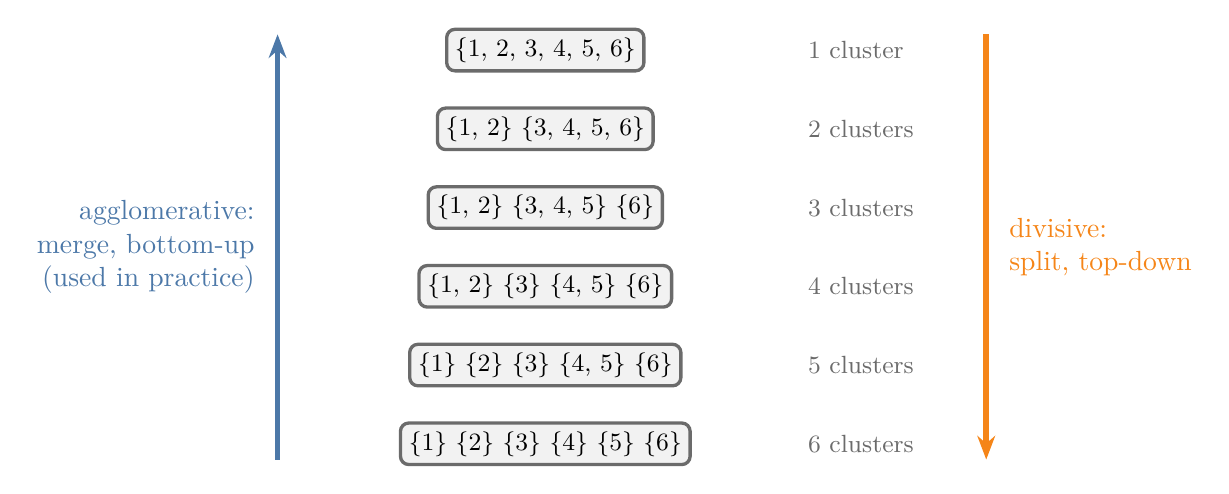
\begin{tikzpicture}[s/.style={draw=cgrey, fill=black!5, rounded corners=3pt, font=\sffamily\small, inner sep=3pt}]
  \foreach \lvl/\txt in {0/{\{1\} \{2\} \{3\} \{4\} \{5\} \{6\}}, 1/{\{1\} \{2\} \{3\} \{4, 5\} \{6\}}, 2/{\{1, 2\} \{3\} \{4, 5\} \{6\}},
                          3/{\{1, 2\} \{3, 4, 5\} \{6\}}, 4/{\{1, 2\} \{3, 4, 5, 6\}}, 5/{\{1, 2, 3, 4, 5, 6\}}} {
    \node[s] (n\lvl) at (0, 1.0*\lvl) {\txt};
    \pgfmathtruncatemacro{\k}{6 - \lvl}
    \node[note, anchor=west] at (3.2, 1.0*\lvl) {\k\ cluster\ifnum\k>1 s\fi};
  }
  \draw[arrow, draw=cblue, line width=2pt] (-3.4, -0.2) -- (-3.4, 5.2) node[midway, left=4pt, align=right, text=cblue, font=\sffamily] {agglomerative:\\merge, bottom-up\\(used in practice)};
  \draw[arrow, draw=corange, line width=2pt] (5.6, 5.2) -- (5.6, -0.2) node[midway, right=4pt, align=left, text=corange, font=\sffamily] {divisive:\\split, top-down};
\end{tikzpicture}
\end{document}
